\documentclass[a4paper, 14pt]{extarticle}%тип документа

%Русский язык
\usepackage[T2A]{fontenc} %кодировка
\usepackage[utf8]{inputenc} %кодировка исходного кода
\usepackage[english,russian]{babel} %локализация и переносы

%отступы 
\usepackage[left=2cm,right=2cm,top=2cm,bottom=3cm,bindingoffset=0cm]{geometry}

%Вставка картинок
\usepackage{graphicx}
\usepackage{wrapfig, caption}
\graphicspath{}
\DeclareGraphicsExtensions{.pdf,.png,.jpg, .jpeg}
\newcommand\ECaption[1]{%
     \captionsetup{font=footnotesize}%
     \caption{#1}}

%Таблицы
\usepackage[table,xcdraw]{xcolor}
\usepackage{booktabs}

%Графики
\usepackage{pgfplots}
\pgfplotsset{compat=1.9}

%Математика
\usepackage{amsmath, amsfonts, amssymb, amsthm, mathtools}

%Заголовок
\author{Подлесный Артём \\ группа 827}
\title{Вопрос по выбору \\ Скин-эффект в полом цилиндре}

\begin{document}
\maketitle

\paragraph*{Цель работы:} исследование проникновения переменного магнитного поля
в медный полый цилиндр.
\paragraph*{Оборудование:} генератор звуковой частоты, соленоид, намотанный на полый цилиндрический каркас из диэлектрика, медный экран
в виде трубки, измерительная катушка, амперметр, вольтметр, осциллограф.

\section*{Краткая теория}

В основе современной электродинамики сплошных сред лежат уравнения Максвелла: 
\begin{equation}
\text{div}\overrightarrow{D} = 4\pi \rho, \text{     }\oint \overrightarrow{D}\overrightarrow{dS} = 4\pi q,
\end{equation} 
\begin{equation}
\text{rot}\overrightarrow{E} = -\dfrac{1}{c}\dfrac{\partial\overrightarrow{B}}{\partial t}, \text{     }\oint \overrightarrow{D}\overrightarrow{dl} = - \dfrac{1}{c}\int \dfrac{\partial\overrightarrow{B}}{\partial t} \overrightarrow{dS} ,
\end{equation} 
\begin{equation}
\text{div} B = 0, \text{   } \oint BdS = 0,
\end{equation}
\begin{equation}
\text{rot} H = \frac{4\pi}{c}j + \dfrac{1}{c}\dfrac{\partial\overrightarrow{D}}{\partial t}  , \text{   } \oint Hdl =\frac{4\pi}{c}I +\dfrac{1}{c}\int \dfrac{\partial\overrightarrow{D}}{\partial t}dS.
\end{equation}

Уравнение (1) — это одна из форм записи закона Кулона. Уравнение (2) —
формулировка закона электромагнитной индукции Фарадея: изменяющееся
во времени магнитное поле порождает вихревое электрическое поле. Уравнение (3) утверждает факт отсутствия магнитных зарядов, и, наконец, уравнение (4) показывает, что магнитное поле порождается не только движущимися
зарядами (первый член в правой части уравнения), но
и изменяющимся во времени электрическим полем. Этот член был введён Максвеллом. Величина $\frac{\partial\overrightarrow{D}}{\partial t}$ по аналогии с $j$ называется плотностью токов смещения.

Рассмотрим электромагнитные волны в проводящей среде. Далее вывод формул будет производится в СИ, так как это лаба, и нужно будет сравнивать получившиеся значения с табличными. Проводимость меди достаточно большая, поэтому в выводе мы пренебрегаем токами смещения. Объемные свободные заряды равны 0 по всему объему проводника. Продифференциировав ур-ние (4) по времени, получим:
\[\text{rot}\dfrac{\partial\overrightarrow{H}}{\partial t} = \sigma\dfrac{\partial\overrightarrow{E}}{\partial t},\]
тк $j = \sigma E$. Взяв rot от обоих частей уравнения (2), и зная, что $\text{rotrot}E = \text{graddiv}E - \Delta E$, и $\text{div} E = 0$, получаем:
\begin{equation}
\Delta E = \mu_0\mu\sigma\dfrac{\partial\overrightarrow{E}}{\partial t}.
\end{equation}

Рассмотрим сначала одномерный случай, представленный на рис. 1.

\begin{wrapfigure}{r}{0.3\textwidth}
\begin{center}
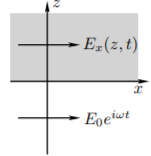
\includegraphics[height=4cm]{teor1.png}
\end{center}
\ECaption{Поле направлено по оси х. Полупространство z>0 заполнено средой с проводимостью $\sigma$, а z<0 -- обычное пространство, с полем, распространяющемся по гармоническому закону.}
\end{wrapfigure}

Будем искать решение (5) в гармоническом виде:
\[E_x(z,t) = E(z)e^{i\omega t}.\] 
После его подстановки в (5) получаем:
\[\dfrac{\partial^2E(z)}{\partial z^2} = i\mu_0\mu\sigma\omega E(z),\]
решение которого ищем в виде $E(z) = Ae^{\alpha x}$. Решая уравнение, получаем общее решение для нашего случая:
\begin{equation}
E_x(z,t) = E_0e^{-\rho z}e^{i(\omega t - \rho z)},
\end{equation}
где $\rho =\sqrt{ \frac{\mu_0\mu\sigma\omega}{2}}$.
Из полученного решения (6) видно, что по мере проникновения переменного
электрического поля с частотой
$\omega$ вглубь проводника фаза
колебаний поля
растёт линейно, а амплитуда убывает по экспоненциальному закону. Такой
закон спадания
характеризуется расстоянием, на
котором амплитуда поля
уменьшается в $e$ раз. Это расстояние называется глубиной проникновения
поля:
\begin{equation}
\delta = \dfrac{1}{\rho}=\sqrt{\dfrac{2}{\mu_0\mu\sigma\omega}}.
\end{equation}
Как видно из этого выражения, с ростом частоты
$\omega$ электрическое поле
всё более «вытесняется»
к поверхности проводника. Это явление называется
скин-эффектом. При выводе зависимости для магнитного поля $H$, выражение будет аналогичным, что несложно показать.

В работе рассматривается полый цилиндр, радиусом $a$ и толщиной стенки $h$. В случае цилиндрического сплошного или полого проводник
а следует решать уравнения, записанные в цилиндрической системе
координат. Их решениями будут функции Бесселя, однако в данном случае нас интересует случай $h\ll a$, что позволяет рассматривать его как плоскопараллельную пластину толщиной $h$. 

\begin{wrapfigure}{l}{0.3\textwidth}
\begin{center}
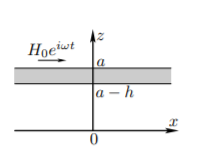
\includegraphics[height=4cm]{teor2.png}
\end{center}
\ECaption{Цилиндр во внешнем магнитном поле.}
\end{wrapfigure}

Теперь, решение ур-ния $\frac{\partial^2E(z)}{\partial z^2} = i\mu_0\mu\sigma\omega E(z)$ будем искать в таком виде: 
\[H(z) = Ae^{\frac{\sqrt{2i}}{\delta}z}+ Be^{-\frac{\sqrt{2i}}{\delta}z}.\]

Это связано с тем, что в данном случае мы рассматриваем конечный слой, а не полупространство. Решение мы ищем для $a-h<z<h$. Запишем граничные условия, как 
\[H(a) = H_0, \text{ } H(a-h) = H_{0c},\]

где $H_0$ - величина поля в соленоиде без экрана, а $H_{0c}$ -- с экраном. Решая получившиеся уравнения, находим решение для граничных условий:
\begin{equation}
\dfrac{H_0c}{H_0} = \dfrac{2}{ak\text{sh}(kh) + \text{ch}(kh)},
\end{equation}
где $k = \frac{1+i}{\delta}$. Соотношение (8) выражает связь между амплитудой магнитного поля
$H_0$ вне проводящего цилиндра радиуса $a$ и толщиной $h$ и амплитудой поля $H_{0с}$ внутри цилиндра. При малых частотах, когда $h\ll\delta$, имеем:
\begin{equation}
\dfrac{|H_{0c}|}{|H_0|}\approx 1 - \dfrac{(\mu_0\sigma ah)^2\omega^2}{8}.
\end{equation}
При больших частотах, когдa $h\gg\delta$, выражение (8) можно записать в виде: 
\[H_{0c} = H_0\sqrt{2} e^{-\frac{h}{\delta}}e^{-(\frac{\pi}{4}+\frac{h}{\delta})},\]
откуда видим, что поле внутри цилиндра запаздывает по фазе на:
\begin{equation}
\psi = \frac{\pi}{4}+\frac{h}{\delta}.
\end{equation}

\section*{Экспериментальная установка}

\begin{figure}[h]
\begin{center}
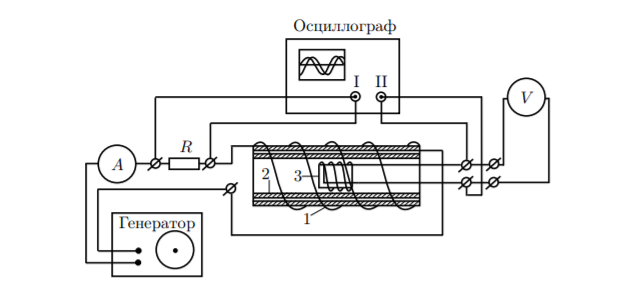
\includegraphics[width=0.9\textwidth]{ust}
\end{center}
\ECaption{Схема экспериментальной установки для
исследования проникновения переменного магнитного поля в медный полый
цилиндр. Для измерения сдвига фаз между током в цепи соленоида и напряжением на измерительной
катушке используется двухканальный осциллограф. На вход одного канала
подаётся напряжение с резистора $R$, которое пропорционально току, а на
вход второго канала — напряжение с измерительной катушки. Радиус цилиндра $a$ = 21 мм, $h$ = 1.3 мм.}
\end{figure}

\section*{Измерение отношения абсолютных величин амплитуд магнитного поля внутри и вне экрана}
С помощью вольтметра «V » мы измеряем действующее значение ЭДС
индукции, которая возникает в измерительной катушке, находящейся в переменном магнитном поле:
\[H_{0c}(t) = H_{0c} e^{i\omega t}.\]

ЭДС индукции в измерительной катушке:
\[\xi_i= -i\mu_0SN\omega H_{0c}e^{i\omega 1}.\]
Обозначим показание вольтметра «V » через $U_k$, тогда
\[U_k = \dfrac{\mu_0SN\omega}{\sqrt{2}}|H_{0c}|.\]
Из этого соотношения следует, что абсолютная величина амплитуды магнитного поля внутри экрана
\[|H_{0c}| \sim \dfrac{U_k}{\omega}\sim \dfrac{U_k}{f}.\]
Но поле внутри экрана
пропорционально полю вне экрана
$H_0$, а
 $H_0 \sim I_A$, где
$I_A$
— показание амперметра «A» в цепи соленоида. Следовательно, амплитуда поля внутри экрана,
приведённая
к единичному току через соленоид
\[|H_0|\sim\dfrac{U_k}{fI_A}.\]
Обозначим величину, пропорциональную $|H_{0с}|$, через $\xi_{0c}$:
\begin{equation}
\xi_{0c} = \dfrac{U_k}{fI_A}.
\end{equation}

Нам теперь необходимо найти амплитуду поля вне экрана при том
же единичном токе через соленоид. Для этого воспользуемся соотношением (9). Как видно из этой формулы, проведя измерения $\xi_{0c}$ в области низких частот (20-100 Гц), и построя по ним график $\xi_{0c}(f^2)$, то экстраполируя его в $f=0$, получаем значение $\xi_0$. 

Отношение
амплитуд магнитного поля внутри экрана
и вне при фиксированной частоте
$f$ будет рaвно
\begin{equation}
\dfrac{|H_{0c}|}{|H_0|} = \dfrac{\xi_{0c}(f)}{\xi_0} = \dfrac{U_k}{fI_a\xi_0}.
\end{equation}
Такой способ измерения
коэффициента ослабления магнитного поля проводящим экраном не требует поддерживать постоянный ток через соленоид
при измерении частотной зависимости этого
коэффициента.

Экспериментальные данные зависимости амплитуды в соленоиде от частоты генератора представлены в таблице 1.
\begin{table}[h!]
\begin{center}
\begin{tabular}{|c|c|c|c|}
\hline
\rowcolor[HTML]{9698ED} 
$f$, Hz & $U_k$, B & $I_A$, mA & $\xi_{0c}$, Ом*с \\ \hline
20      & 0.0281   & 114.8     & 0.0122           \\ \hline
\rowcolor[HTML]{9698ED} 
30      & 0.042    & 115.1     & 0.0121           \\ \hline
40      & 0.0556   & 115.3     & 0.0120           \\ \hline
\rowcolor[HTML]{9698ED} 
50      & 0.069    & 115.4     & 0.0119           \\ \hline
60      & 0.082    & 115.4     & 0.0118           \\ \hline
\rowcolor[HTML]{9698ED} 
70      & 0.0947   & 115.4     & 0.0117           \\ \hline
80      & 0.107    & 115.3     & 0.0116           \\ \hline
\rowcolor[HTML]{9698ED} 
90      & 0.1187   & 115.2     & 0.0114           \\ \hline
100     & 0.13     & 115.2     & 0.0113           \\ \hline
\end{tabular}
\ECaption{Зависимость $\xi_{0c}(f)$. } 
\end{center}
\end{table}

По этим данным строим график зависимости из соотношения (9) на рис.4.

\begin{figure}[h!]
\begin{center}
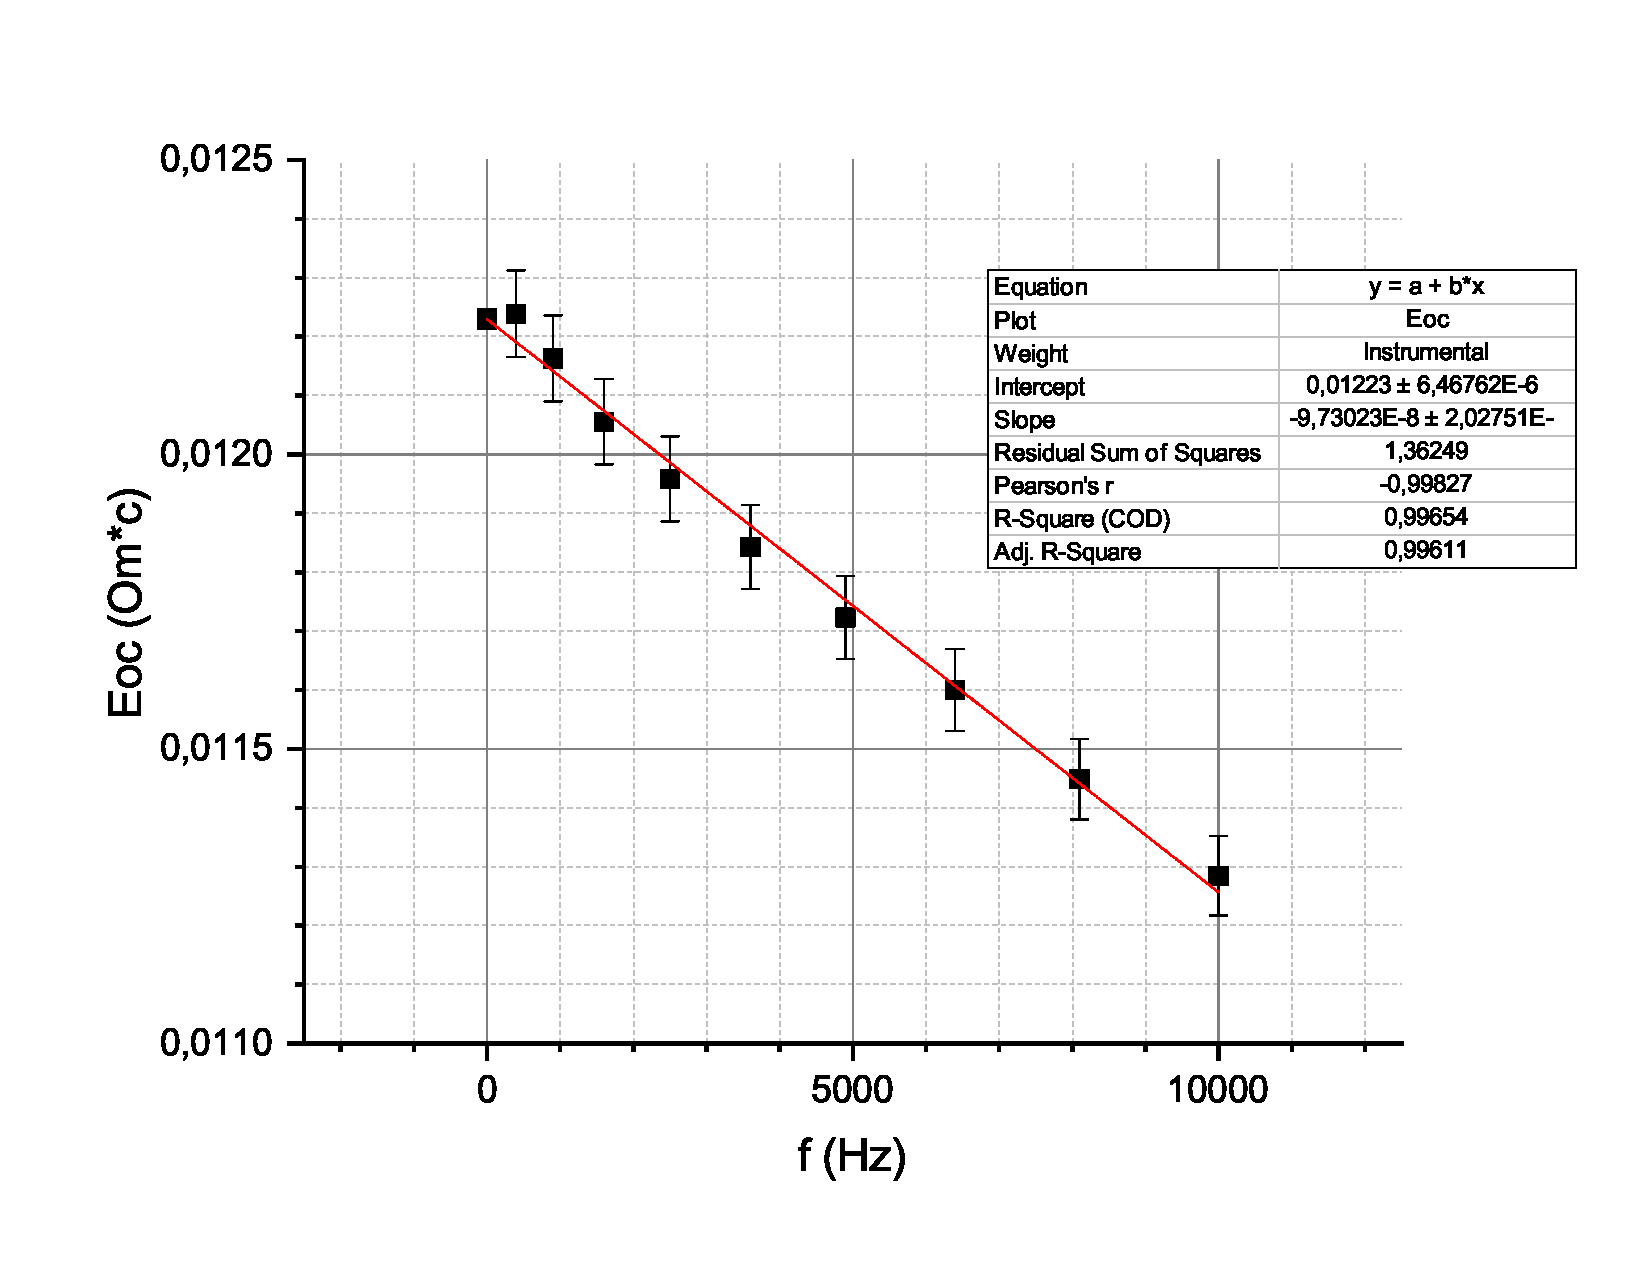
\includegraphics[width=0.9\textwidth]{E0}
\end{center}
\ECaption{График зависимости $\xi_{0c}(f^2)$. На нем представлена таблица со всеми необходимыми данными, а так же отмечена точка пересечения прямой с осью ординат, соответствующая амплитуде вне цилиндра.}
\end{figure}

Таким образом, получаем искомое значение вместе с погрешностью:
\[\xi_0 = 12.23 \pm 0.02 \text{ мОм}\cdot c.\]

Получив это значение, по формуле (12) мы сможем определить коэффициент ослабления магнитного поля при фиксированной частоте.

\section*{Определение проводимости материала экрана}

По формуле (10), сняв зависимость разности фаз между полем внутри соленоида и снаружи на высоких частотах (100 Гц - 19 кГц), можно определить проводимость металла по углу наклона прямой, заданной зависимостью $\psi(\sqrt{f})$. При снятии этой зависимости необходимо учитывать, что сигнал, подающийся на осциллограф (канал 2) пропорционален производной по времени магнитного поля, поэтому посчитанную разность фаз необходимо уменьшить еще на $\frac{\pi}{2}$. Так же, для следующего этапа работы необходимо было посчитать параллельно с фазами еще и зависимость $\xi_{0c}(f)$. Все эти данные представлены на таблице 2.

\begin{table}[h!]
\begin{center}
\begin{tabular}{|c|c|c|c|c|c|}
\hline
\rowcolor[HTML]{9698ED} 
$f$, kHz & $U_k$, B & $I_A$, mA & $x_{\pi}$, cm & $\Delta x$, cm & $\psi/\pi$ \\ \hline
0.1      & 0.13     & 115       & 4.5           & 2.8            & 0.122      \\ \hline
\rowcolor[HTML]{9698ED} 
0.5      & 0.3086   & 114.7     & 4.6           & 4              & 0.370      \\ \hline
1        & 0.331    & 114.2     & 4.5           & 4.4            & 0.478      \\ \hline
\rowcolor[HTML]{9698ED} 
2        & 0.3396   & 115.4     & 4.6           & 4.6            & 0.500      \\ \hline
4        & 0.3336   & 114.1     & 5.6           & 6.4            & 0.643      \\ \hline
\rowcolor[HTML]{9698ED} 
6        & 0.333    & 112.5     & 3.8           & 4.4            & 0.658      \\ \hline
8        & 0.32     & 109.3     & 5.7           & 6.3            & 0.605      \\ \hline
\rowcolor[HTML]{9698ED} 
10       & 0.308    & 105.7     & 4.4           & 4.8            & 0.591      \\ \hline
12       & 0.294    & 99.8      & 3.4           & 4.5            & 0.824      \\ \hline
\rowcolor[HTML]{9698ED} 
14       & 0.282    & 94        & 3             & 4              & 0.833      \\ \hline
16       & 0.27     & 87.1      & 2.8           & 4              & 0.929      \\ \hline
\rowcolor[HTML]{9698ED} 
18       & 0.284    & 85.7      & 5             & 7.2            & 0.940      \\ \hline
19       & 0.277    & 80.7      & 4.8           & 7.2            & 1.000      \\ \hline
\end{tabular}
\ECaption{Зависимость амплитуды поля в соленоиде и разности фаз (деленой на пи) между внешним и внутренним магнитными полями от частоты. В работе предполагалось снимать зависимость и при более выоких частотах, однако на той установке, на которой я делал, при смене регулировки на более высокую частоту, происходил сбой, который при мне не смог устранить даже лаборант. Однако результаты все еще достоверные, так что это не является большой проблемой.}
\end{center}
\end{table}

Остается построить график зависимости (10), и по углу наклона прямой, проходящей через нулевую точку ($\psi(0) = \frac{\pi}{4}$), и достаточно высокие частоты, определить проводимость меди. Он изображен на рис.5.

\begin{figure}[h!]
\begin{center}
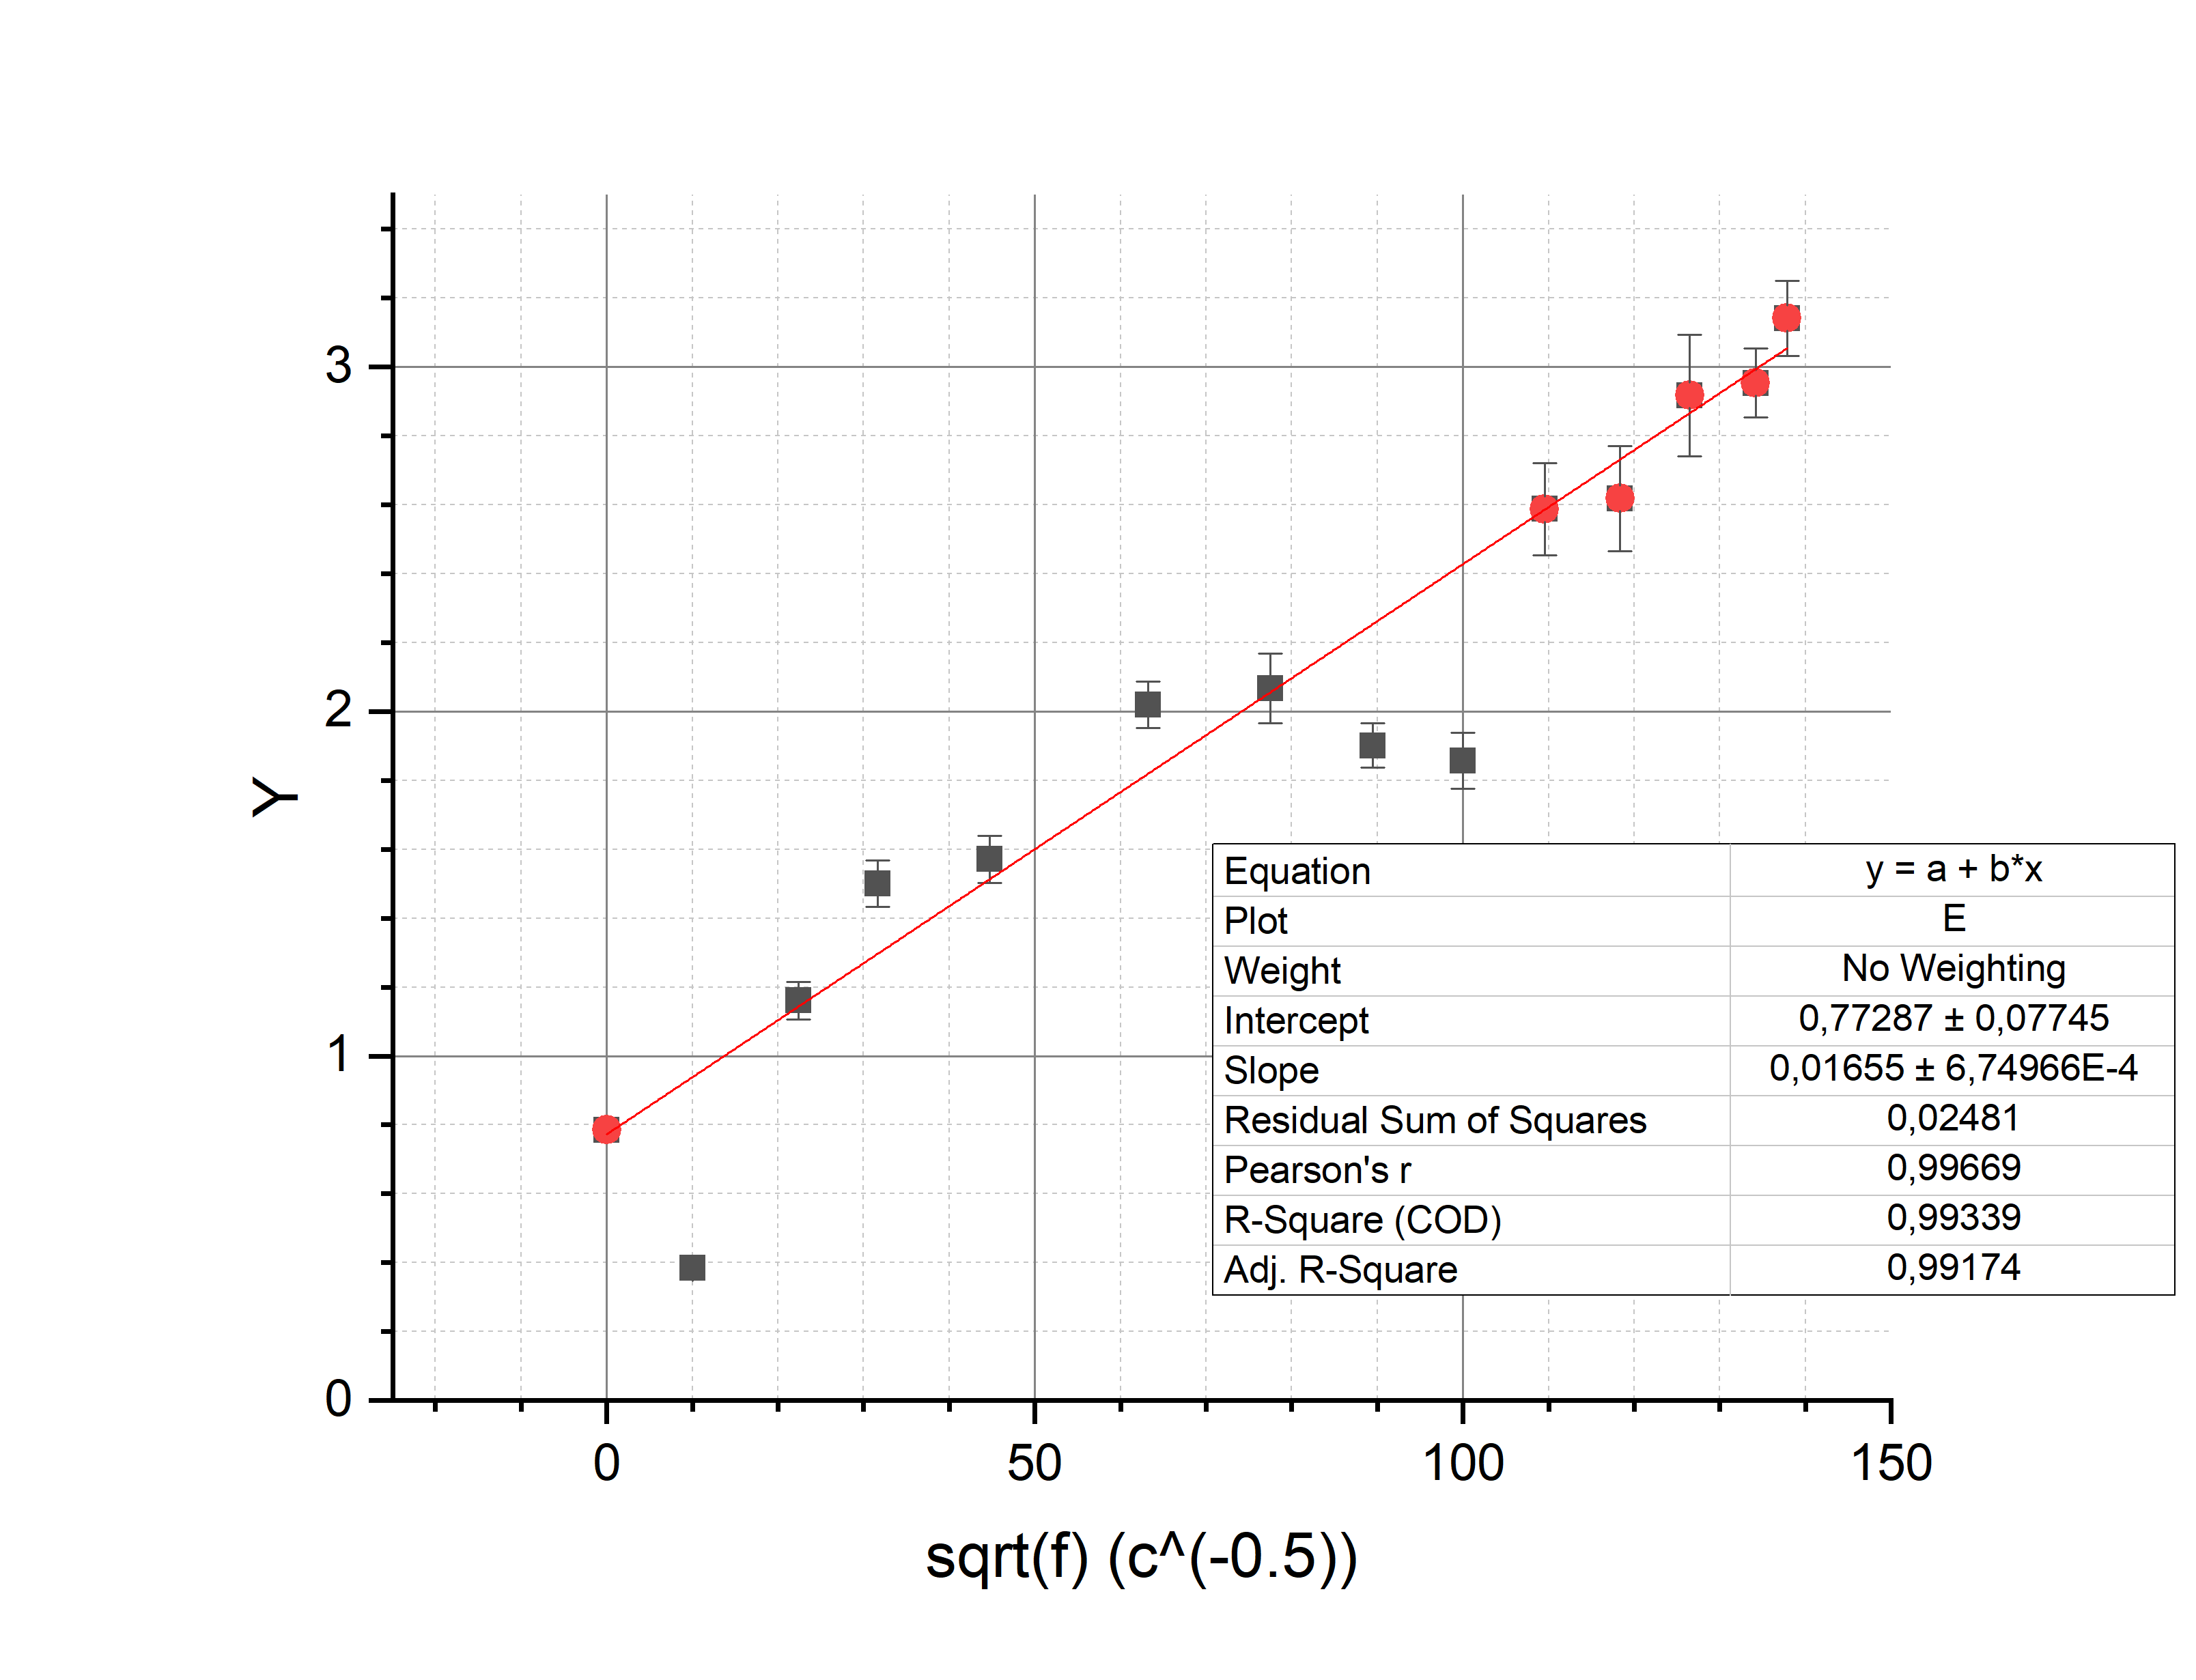
\includegraphics[width=0.9\textwidth]{f}
\end{center}
\ECaption{График зависимости $\psi(\sqrt{f})$. Точки, по которым проводилась прямая, окрашены другим цветом (в цветной версии - красным). Здесь так же видны 2 точки, которые сильно выбиваются из общей зависимости - вероятнее всего, это произошло из-за того, что в первое измерение я забыл их померить, а вернувшись назад, столкнулся с эффектом гистерезиса. Я решил их оставить, чтобы показать, что в данной работе он большой. }
\end{figure}

Из графика получается его коэффициент наклона:
\[\alpha = 0.0166\pm0.0007 \text{ c}^{\frac{1}{2}}.\]
С учетом этого, соотношение для проводимости из (10) записывается так:
\[\sigma = \dfrac{\alpha^2}{\mu_0\pi h^2} = (43.2 \pm 0.7)\times 10^6 \text{ Ом}^{-1}.\]

Табличное значение для меди колеблется в районе $55\times 10^6 \text{ Ом}^{-1}$. С учетом того, что технология изготовления труб оказывает заметное
влияние на её электропроводимость, электропроводимость меди нашей трубы отличается от табличного значения в область заниженного значения. Поэтому полученное значение вполне можно считать достоверным.
 
\section*{Проверка применимости используемых формул}

Используя полученное значение для амплитуды поля вне цилиндра, с помощью формулы (12) можем получить зависимость коэффициента ослабления от корня из частоты генератора. Эту же зависимость можно получить теоретически, используя формулу (8) и экспериментально определенное значение проводимости меди. Так как получать явное выражение для модуля (8) чересчур трудоемко, эта зависимость была снята с использованием обсчитывающих программ (вольфрама). После обе зависимости были нанесены на один график, изображенный на рис. 6.

\begin{figure}[h!]
\begin{center}
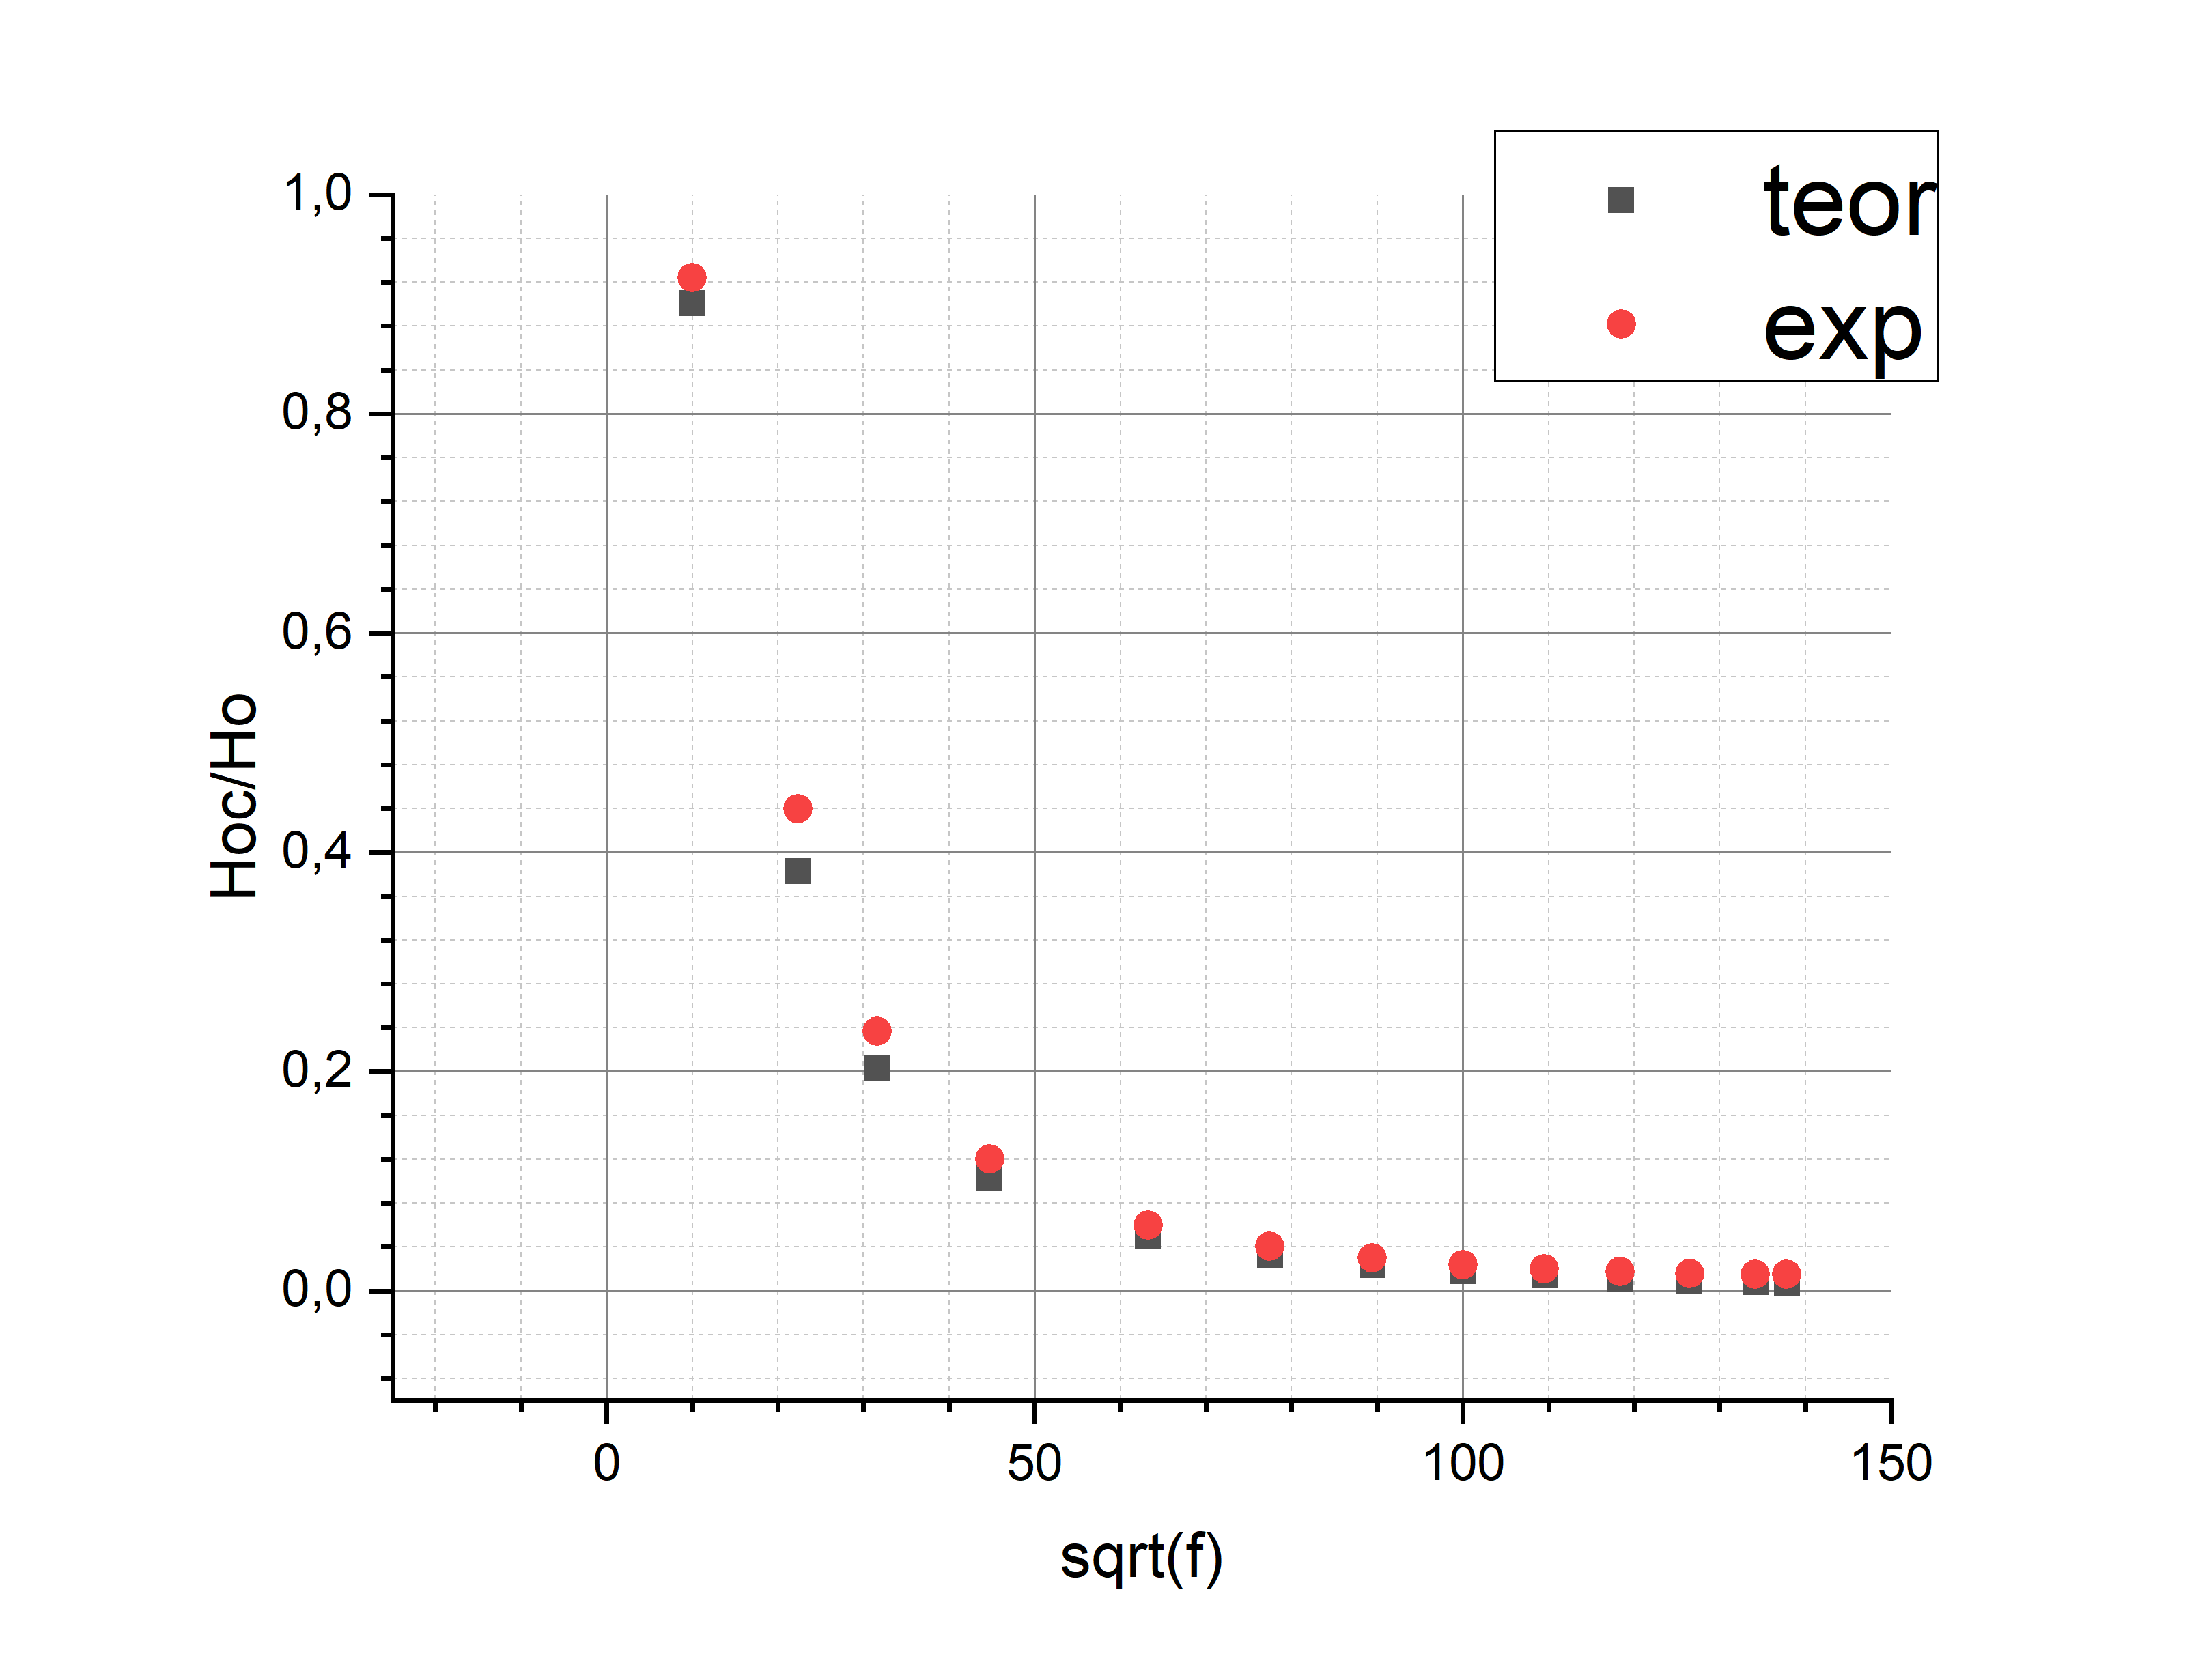
\includegraphics[width=0.9\textwidth]{te}
\end{center}
\ECaption{График зависимостей $\frac{|H_{0c}|}{|H_0|}(\sqrt{f})$, полученных экспериментально и теоретически (обозначены на самом графике). }
\end{figure}

Как видно из графиков, значения практически совпадают (основная погрешность связана с определением проводимости меди). Таким образом, такой метод определения коэффициента ослабления магнитного поля можно считать достоверным. 

Теперь необходимо проверить, выполняются ли условия $\frac{h}{\delta}\ll 1$, или $\frac{h}{\delta}\gg$ для соответствующих частот, с которыми мы работали. Для этого был произведен расчет глубины проникновения $\delta$ с помощью посчитанной экспериментально проводимости меди $\sigma$ для двух частот — 50 Гц — характерная низкая частота, $10^5$ Гц - характерная высокая. Результаты на таблице 3:
\begin{table}[h!]
 \begin{center}
\begin{tabular}{|c|c|c|}
\hline
\rowcolor[HTML]{9698ED} 
$f$, Hz & $\delta$, mm & $\frac{h}{\delta}$  \\ \hline
50      & $10.8\pm0.3$     & 0.12 \\ \hline
\rowcolor[HTML]{9698ED} 
$10^5$  & $0.24 \pm 0.01$     & 5.38 \\ \hline
\end{tabular}
 \end{center}
\end{table}

Видно, что условия для использования формул (9) и (10) выполняются в каждом конкретном случае.

 \section*{Вывод}
Было исследовано проникновение переменного магнитного поля в медный полый цилиндр. Показано, что с достаточно хорошей точностью, (зависящей от установки), с можно определить такие важные параметры, как ослабление магнитного поля и проводимость меди, без необходимости поддерживать постоянный ток через цилиндр. В целом скин-эффект в полом цилиндре играет огромную роль в электротехнике. Например при передаче высокочастотного тока нет необходимости делать провода сплошными, а можно сделать их полыми, так как все равно ток будет проходить по скин-слою. Это особенно существенно при передаче тока на большие расстояниях, когда играет роль вес конструкции и расход металла. 









\end{document}